\documentclass[12pt]{article}

\usepackage[a4paper,margin=0.5in]{geometry}
\usepackage[square,numbers,sort&compress]{natbib}
\usepackage[utf8]{inputenc} % allow utf-8 input
\usepackage[T1]{fontenc}    % use 8-bit T1 fonts
\usepackage{hyperref}       % hyperlinks
\usepackage{url}            	% simple URL typesetting
\usepackage{booktabs}     % professional-quality tables
\usepackage{amsfonts}     % blackboard math symbols
\usepackage{nicefrac}       % compact symbols for 1/2, etc.
\usepackage{microtype}    % microtypography
\usepackage{amsmath}
\usepackage{algorithm}
\usepackage[noend]{algpseudocode}

\usepackage{graphicx}
\newcommand{\bigo}[1]{{\cal O}\left(#1 \right)}
\newcommand{\p}{\mathrm{P}}
\newcommand{\vect}[1]{\mathbf{#1}}
\newcommand{\indp}[2]{#1 \perp\!\!\!\perp #2}


\begin{document}
\thispagestyle{empty}
\begin{center}

\textbf{DS-GA 1018.001 Probabilistic Time Series Analysis\\
Homework 1}
\end{center}

\noindent \textbf{Due date: Sept. 29, by 6pm}\\
\\
\noindent \textbf{Problem 1. } (10pt) Given the graphical model below, write down the factorization for $P(x_{1:10})$. What happens with the distribution when conditioning on $x_3$?
\begin{figure}[h!]
\centering
\vspace{-1mm}
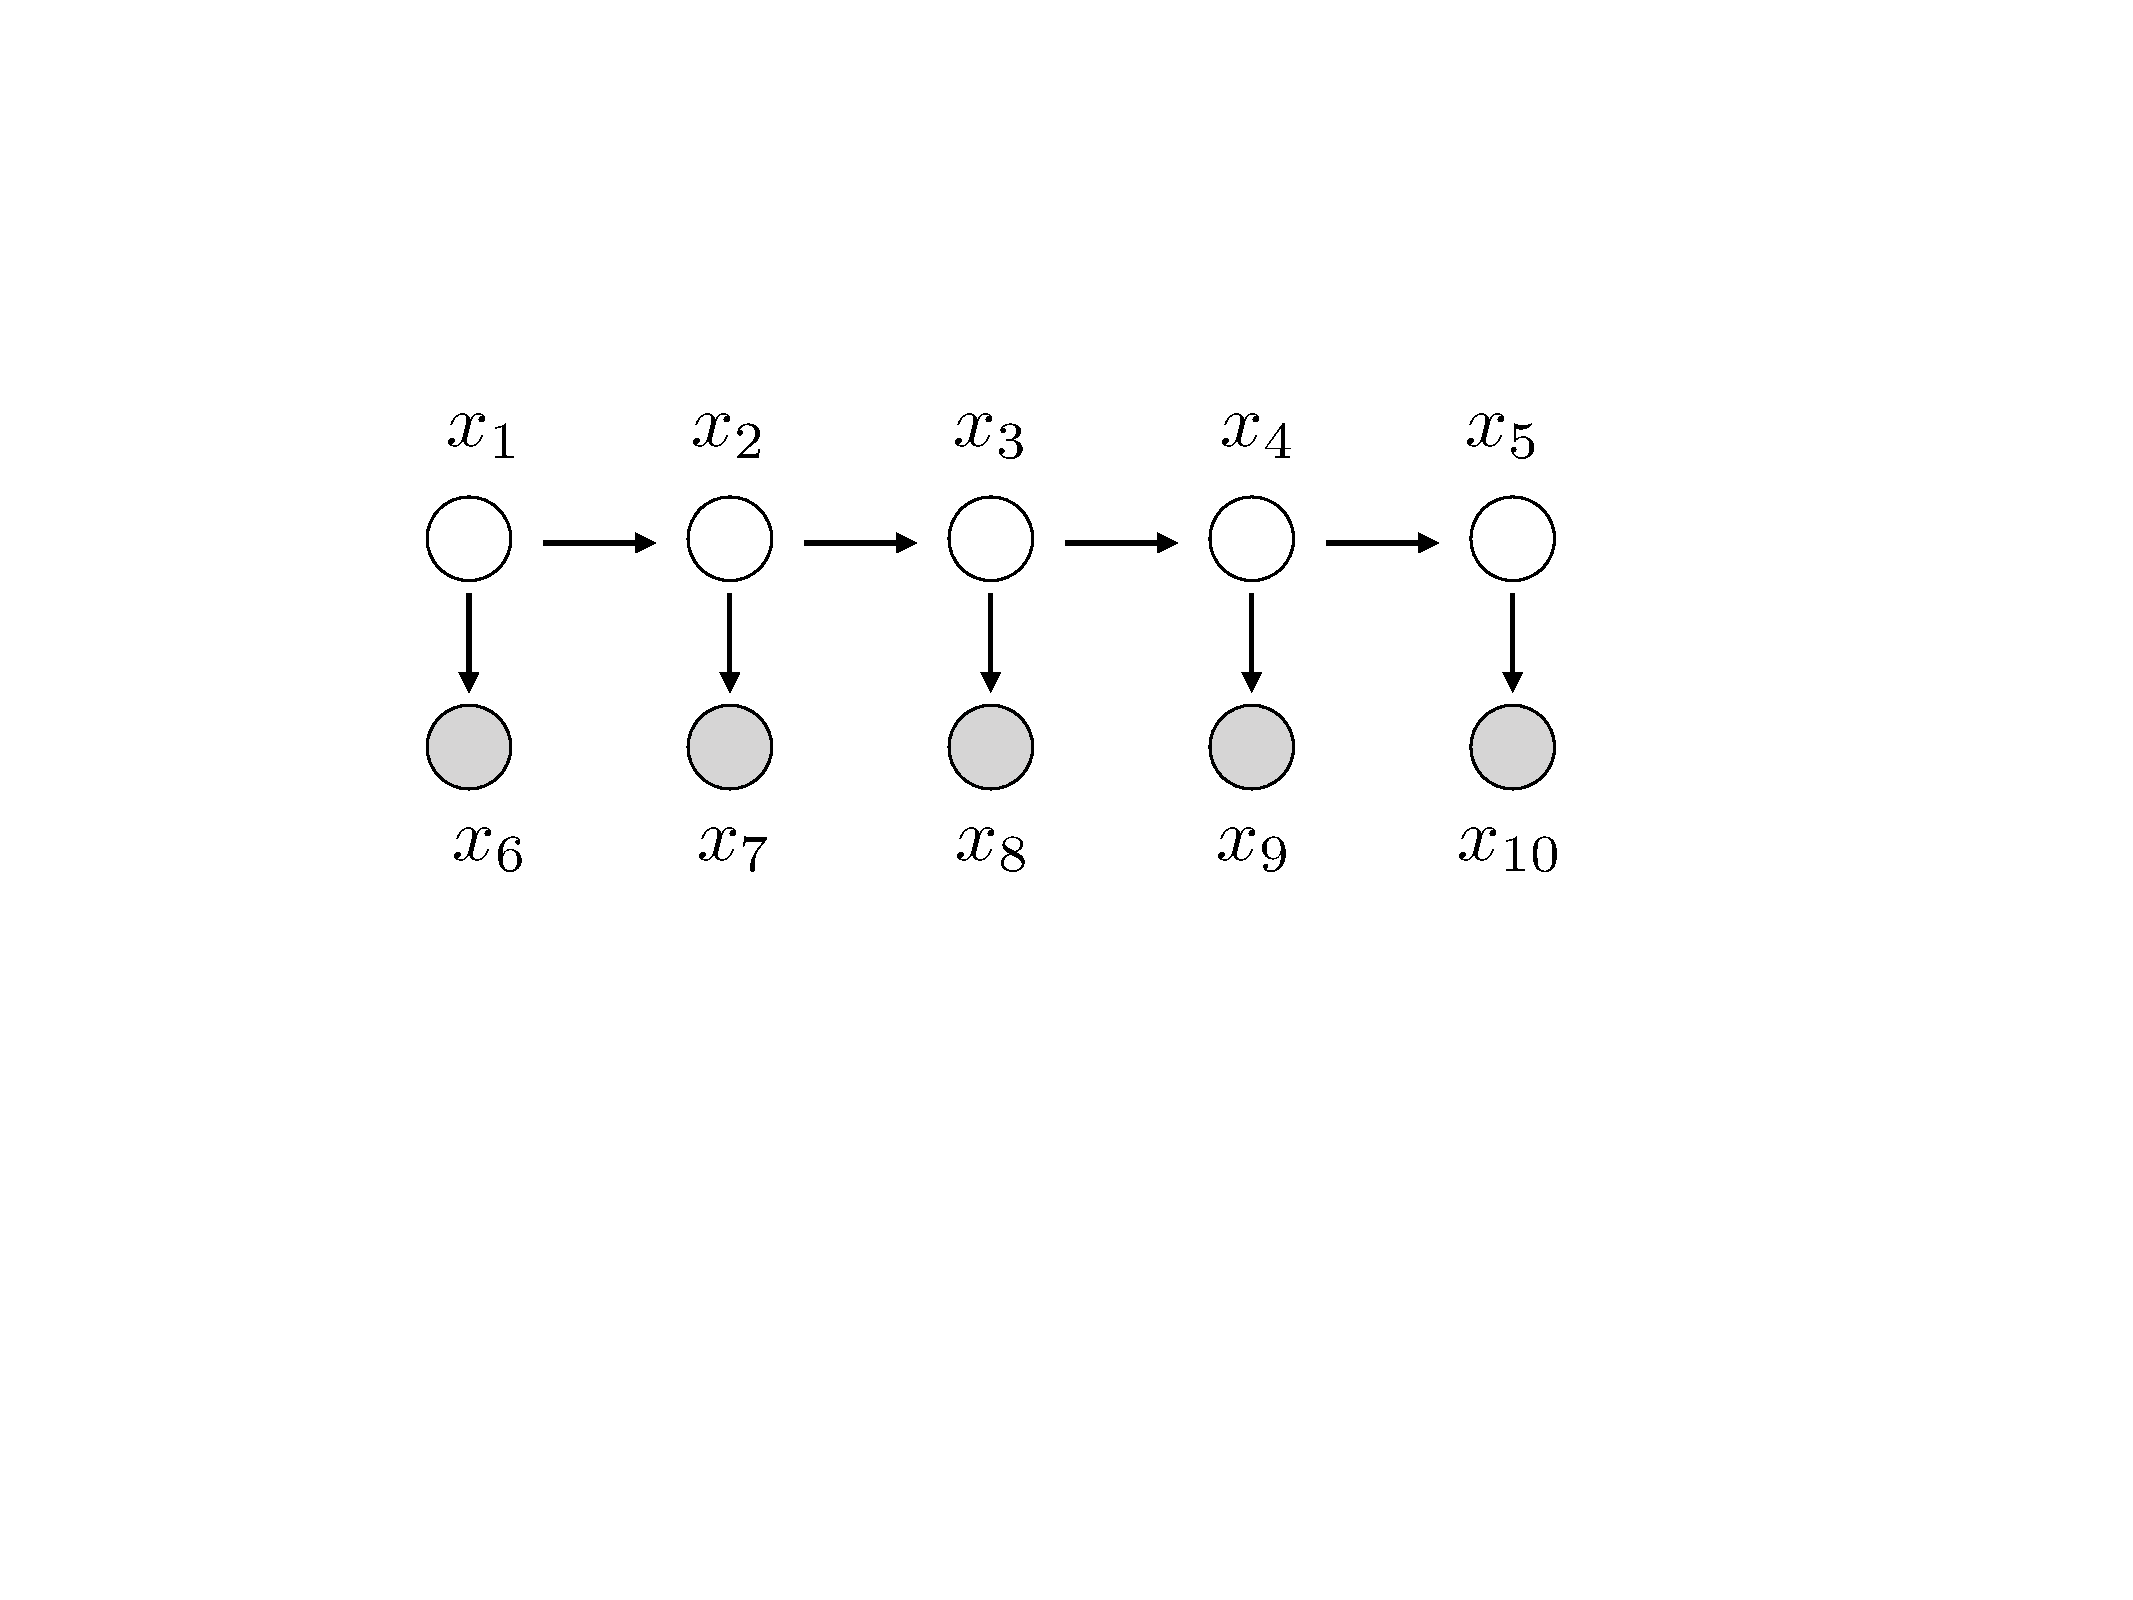
\includegraphics[width=4.5in]{gmhw1.pdf}
\end{figure}


\noindent \textbf{Problem 2. }  (10pt) Consider the \emph{sample mean} of a stationary time series  $x_t$, defined as:
\begin{equation}
\hat{\mu} = \frac{1}{T} \sum_t x_t.
\end{equation}
Compute the variance of this estimate $Var[\hat{\mu}]$, as a function of $T$, and the autocovariance function $\gamma(h)$.\\
\emph{Hint: The empirical mean is also a linear combination of random variables, so you can use the formula for the covariance of linear combinations of random variables from the lecture. }\\

\noindent \textbf{Problem 3. } (10pt) Confidence bounds for the autocorrelation function: 
show that the variance of the empirical ACF for white noise with variance $\sigma^2$ estimated given $T$ data points is $\frac{1}{T}$.\\
\emph{Hint: Use theorem A.7 from Shumway, and  Stoffer  (yellow book, pdf on brightspace); alternatively, you can just show it numerically by plotting empirical estimates of the ACF as a function of T. }\\

%\noindent \textbf{Problem 3. } (10pt)
%For an MA(1), $x_t = w_t + \theta w_{t-1}$ show that the autocorrelation function $|\rho_x(1) | \leq 0.5$, for all $\theta$. 
%For which values $\theta$ is it maximum/minimum?\\

\noindent \textbf{Problem 4.} (5pt+5pt) Identify the following models as $\mathrm{ARMA}(p,q)$:
\begin{itemize}
\item $x_t = 0.8 x_{t-1} - 0.15 x_{t-2} + w_t - 0.3 w_{t-1}$
\item $x_t =  x_{t-1} - 0.5 x_{t-2} + w_t - w_{t-1}$
\end{itemize}
\emph{Note: watch out for parameter redundancy!}\\

%\noindent \textbf{Problem 5.} (5pt) Having observed a sequence  $\{x_1,x_2... x_t \}$ we are trying to predict a future observation $x_{t+h}$, with $h\geq1$.
%How well / far can one predict into the future if the data comes from a a) MA(3) and b) AR(1) model. \\
%\emph{Hint: think of the functional form of the optimal estimator and/or the corresponding graphical model.}\\

\noindent \textbf{Problem 5.} (10pt) Given the AR(2) process with $P(B) = (1-0.2B)(1-0.5B)$, what is $\rho(h)$? 
 Check your analytical solution against an empirical estimate obtained using the code from the lab.\\
\emph{Hint: Difference equations + initial conditions.}\\

\end{document}